\documentclass[10pt]{article}
\usepackage{graphicx} % Required for inserting images
\usepackage{subcaption}
\usepackage{float}
\usepackage[T1]{fontenc}
\usepackage[utf8]{inputenc}
\usepackage{lmodern}
\usepackage[english]{babel}
\usepackage[autostyle]{csquotes}

\usepackage{comment}

\usepackage[backend=biber,style=authoryear]{biblatex}
\addbibresource{bibliography.bib}

\title{Image Classification on Satellite Imagery For Sustainable Water Harvesting Placement in Indigenous Communities of Northern Tanzania}
\author{Roshan Taneja, Ms. Kayla Holman}
\date{December 2024}

\begin{document}

\maketitle

\begin{abstract}
Hello this is the abstract, 300 words or less, one paragraph, and should detail the whole project [DO THIS ONCE YOU WRITE THE WHOLE PAPER]
\end{abstract}

\section{Introduction}

\subsection{Background and Context}

According to the United Nations, one in four people cannot access clean water (\autocite{United_Nations}). One such community is the Maasai in the Monduli District of Tanzania. They walk over nine hours daily to fetch water and face climate change and land deforestation challenges. Floods and droughts are more frequent and severe, and traditional water sources, such as rivers and springs, dry up. Annual rainfall in Tanzania is equal to or higher than in the US, yet they face challenges in accessing water. The community has been deploying water harvesting units along the main highway, which currently helps less than 4000 people, but only for short periods. The impact of even one water harvesting unit has been validated. The challenge is that over 30,000-40,000 Maasai live across hundreds of square miles without highways and infrastructure like electricity or water. We need a better technique to identify the living locations, assess the density, and pick the right water harvesting solution that balances cost, ease of deployment, and sustainability. This paper takes the first step in identifying the living locations across hundreds of square miles using satellite images, machine learning, and image classification models. If this approach has high precision, it can be expanded to many regions for water resource planning and management opportunities.  There is a need for sustainable water management solutions to support communities like the Maasai and other areas of Africa.

\begin{figure} [H]
    \centering
    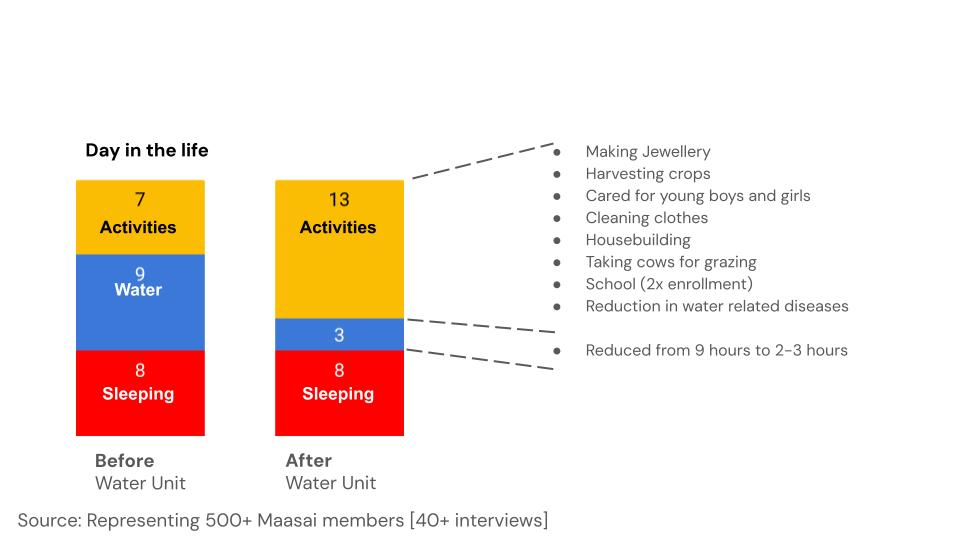
\includegraphics[width=1\linewidth]{images/beforeandafterwhu.jpg}
    \caption{Before and after the Water Harvesting Unit: Doubled the time spent on economic, social, and agricultural activities}
    \label{fig:bef_aft_results}
\end{figure}

The first water harvesting unit of 100K liters directly impacted the community. Specifically, kids have started coming to school more often, and there is higher enrollment of students. Women have seen reduced time spent walking to fetch water and are using the extra time for social, agricultural, and economic activities. Reduced walking from nine to two hours a day (Fig~\ref{fig:bef_aft_results}). 

Given the impact, multiple additional projects have been executed, including deploying a 30+K liter solution serving the Nanja village and a water filtration system in Engirgiri that cleans water collected in a man-made pond that catches rainwater for use by the local Maasai community.






\subsection{Problem Statement and Rationale}

To support water harvesting solutions for 30,000-50,000 Maasai, we needed to identify the best places to locate them across 300-500 square miles. We can identify the best water harvesting solutions based on the population's density distribution. However, the government does not provide accessible maps of the Maasai's location. To design and plan solutions at scale, we decided to see if we could use satellite images and image classification to create a population map and validate the maps with local community involvement.


% The next step would be identifying the best locations for placing the water harvesting solutions.








\subsection{Scope and Limitations}



uhh something here?





\subsubsection{Unique Structure and Materials of Bomas}

\begin{figure} [H]
    \centering
    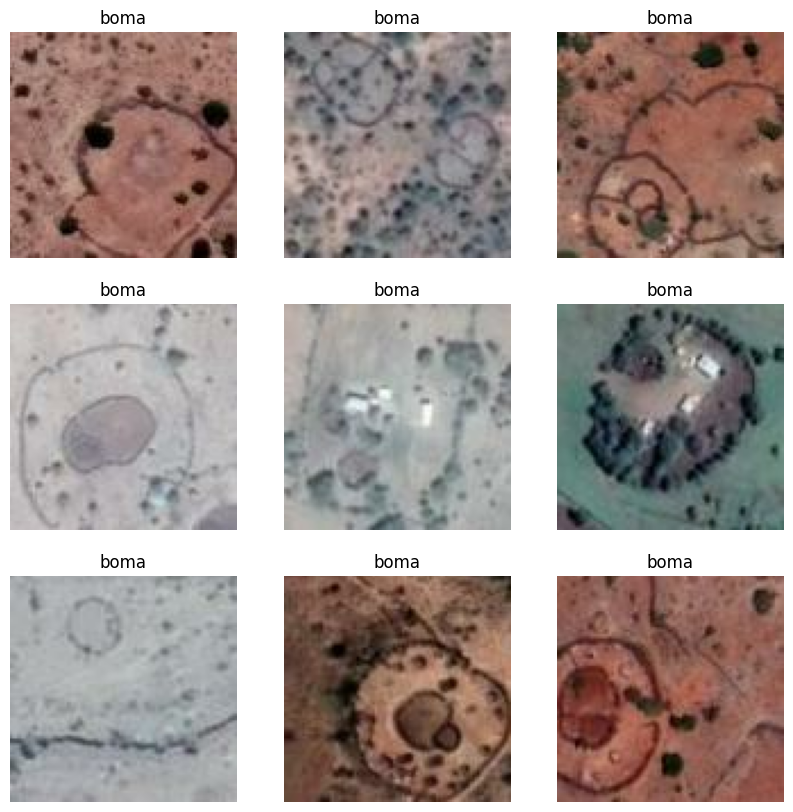
\includegraphics[width=0.8\linewidth]{images/types of bomas.png}
    \caption{Example of Variation in Landscape, Vegetation and Structure}
    \label{fig:types_of_bomas}
\end{figure}

Due to their polygamous nature, familial groups live together in large units called "Bomas." A Boma is a unique structure that is difficult to classify. There is no precise size to a Boma, but it usually consists of multiple small huts, a section for keeping goats and cows safe at night. There are a few characteristics that define a Boma. An outer barrier, usually made from rough bushes. Inside, there may be trees or other structures, such as shelters. At the center will be a smaller circle, also created with bushes, where cattle stay. These Bomas can house 10 to 50 people and sometimes be squares or other shapes, even open ones. Families who own cattle create an inner or outer circle or circles with other things, such as trees. Another issue is the contrast of the bushes with the environment, sometimes not showing up. (Fig~\ref{fig:types_of_bomas})

\subsubsection{Techniques Considered}

In evaluating three different methods for our project, we considered YOLOv7, OpenCV, and TensorFlow. YOLOv7, though highly optimized for speed and accuracy with minimal background detection errors, presented significant challenges. It proved difficult to integrate with Jupyter notebooks(\autocite{s23135849}). It performed inadequately with objects of varying sizes and shapes—critical for our project—and suffered from limited community support(\autocite{IJERTV10IS060287}), maintained by a small team. While boasting extensive community support and customizable settings, OpenCV was deemed overly complex for our beginner-level proficiency, featuring a steep learning curve(\autocite{9174593}).

Conversely, TensorFlow appeared as the optimal choice, balancing accessibility as an open-source tool and compatibility with Python and JavaScript, which is crucial for integrating with Google Earth Engine (GEE).
Despite its higher resource consumption and slower performance, TensorFlow's regular updates and new features make it the most suitable framework for our needs. It provides the necessary tools and support for successful project execution.

\subsection{Objectives}

This research project aims to optimize the placement of water harvesting solutions based on population density and natural water sources. To generate a population density map, we want to use satellite data to detect these uniquely shaped Bomas across selected regions. This data will help identify critical locations for deploying the appropriate water solutions. The options for enhancing water accessibility include large units for housing groups, such as installing communal rainwater harvesting units to serve large groups of Bomas and creating larger-scale rainwater collection systems, such as ponds or dams, to benefit entire communities, especially in more densely populated areas.

\section{Methods}



\subsection{Data}

\subsubsection{Collection}

We considered two different sources for our training data. One was the Copernicus Institute website for the Copernicus Satellites and Google Earth Engine (GEE). We settled on GEE because writing a script to generate the training data from just a few points on a map was easier. We started with 2000 photos of Bomas and 500 photos of the environment (Omits a Boma). The accuracy was around 30\%, far below the required standards. The model needed help with a few problems. First, The color of the Boma circle blended in too well with the environment. Second, There wasn’t enough data to train the AI.


\subsubsection{Augmentation}

We realized that the images could be superimposed, meaning we could rotate and flip them to create more training data for the model. Using this new information, we generated 6,000 more photos of Bomas and 1500 more images of the environment. With this new model trained at 10,000 images, the accuracy skyrocketed to 93\%. Because these "Bomas" are often disguised and varied, more training would not increase the accuracy further. The model plateaus with the current constitution at a certain point due to the extreme shape, color, and size variation. Toggling with filters, cropping, grayscale, or increasing the contrast did not impact the accuracy. Perhaps more fine-tuning is necessary, but it's unlikely to change performance significantly.

\subsection{Model Training}


\subsection{Model Testing}



\subsection{Spacial Coordinate Extraction}



\section{Results}



\section{Discussion}

\subsection{Key Findings}

\subsection{Limitations of Outputs}

\subsection{Implications and Significance}

\subsection{Community Involvement}



\section{Conclusion}

\section*{Acknowledgement}

\printbibliography

\end{document}
